\documentclass[ngerman,a4paper]{report}
\usepackage[english,ngerman]{babel}
\usepackage[T1]{fontenc}
\usepackage[utf8]{inputenc}
\usepackage{geometry}
\usepackage{hyperref}
%\usepackage{MyriadPro}
%\usepackage{MinionPro}
\usepackage{graphicx}
%\geometry{verbose,tmargin=3cm,bmargin=3cm,lmargin=3cm,rmargin=3cm}
\usepackage{listings}
\usepackage{paralist}
\usepackage{stmaryrd}
\usepackage{color}
%\usepackage{floatflt}
\usepackage{amsmath}
%\usepackage{amssymb}
\usepackage{float}
\definecolor{dkgreen}{rgb}{0,0.6,0}
\definecolor{gray}{rgb}{0.5,0.5,0.5}
\definecolor{mauve}{rgb}{0.58,0,0.82}
\lstset{language=C,
numbers=left,
numberstyle=\tiny\color{gray},
stepnumber=1,
numbersep=5pt,
%basicstyle=\tiny,
%frame = single,
tabsize =2,
breaklines = true,
breakatwhitespace = false,
keywordstyle=\color{blue},          % keyword style
commentstyle=\color{dkgreen},       % comment style
stringstyle=\color{mauve},         % string literal style
literate=%
{Ö}{{\"O}}1
{Ä}{{\"A}}1
{Ü}{{\"U}}1
{ß}{{\ss}}2
{ü}{{\"u}}1
{ä}{{\"a}}1
{ö}{{\"o}}1
}

\selectlanguage{english}

\renewcommand{\familydefault}{\sfdefault}

 
\author{Hinnerk van Bruinehsen\\Tobias Höppner\\Tobias Famulla}
\title{Lecture Notes\\\Huge{Distributed System}}
\date{SoSe 2013}

\begin{document}
\maketitle
\tableofcontents

\chapter{Verteilte Systeme/Distributed Systems}
\section{Orga}
VL Di 10-12 (nicht am 23.04.)\\
Ue Do 10-12\\

\subsection{Elektisches}
\begin{compactitem}
\item (kvv)
\item Website AG
\item Sakai
\end{compactitem}

\subsection{Übungen}

\begin{compactitem}
\item ca. 5 Übungsblätter, 14-tägig
\item Vorträge in Gruppen über \glqq verteilte Systeme\grqq
\end{compactitem}

\subsection{Material/Inhalt}
\begin{compactitem}
\item[1. Hälfte] Distributed Systems (Tanenbaum, van Steen)
	\begin{compactitem}
	\item Architektur
	\item Prozesse
	\item Kommunikation
	\item Namen
	\item Synchronisation
	\item Konsistenz
	\item Replikation
	\item Fehlertoleranz
	\end{compactitem}
\item[2. Hälfte] Distributed Algorithms (Nancy Lynch)
	\begin{compactitem}
	\item synchronous network algorithms
	\item network models (leader election, shortest path, distributed consensus, byzantine agreement)
	\item asynchronous network algorithms (shared memory, mutual exclusion, resource allocation, consensus)
	\item timing
	\item network resource allocation
	\item failure detectors
	\end{compactitem}
\end{compactitem}

\chapter{Distributed Systems}
\textbf{Def:} A distributed System is a collection of independent computers that appears to it's users as a single coherent system.

Characteristics:\\
\begin{compactitem}
\item autonomous components
\item appears as single system
\item communication is hidden
\item organisation is hidden \\(could be high-performance mainframe or sensor net)
\item heterogenous system offers homogenous look/interface
\end{compactitem}

Objectives:\\
\begin{compactitem}
\item provide resources (printer, storage, computing)
\begin{compactitem}
\item share in a controlled, efficient way
\item grant access\\
$\Rightarrow$ connect users and resources
\end{compactitem}

\end{compactitem}

Transparency:\\
hide the fact that processes and resources are physically distributed.

Types of transparancy:\\
\begin{compactitem}
\item[access] hide differences in representation and how a resource is accessed
\item[location]
\item[migration] move ressources
\item[relocation] move ressources while using
\item[replication]
\item[concurrency]
\item[failure]
\end{compactitem}

transparancy is desireable, but not always perfectly possible

tradeoff between transparancy and complexity, maintainablility and performance

\textbf{Open System}

\begin{compactitem}
\item service interfaces specified using Interface Definition Language (IDL)
\item service specification as text
\end{compactitem}

\textbf{Scalability} is an important property

\begin{compactitem}
\item scalable in size (number of nodes)
\item scalable in geographic spread
\item scalable in administration
\end{compactitem}

\textbf{Problems}

\begin{compactitem}
\item centralized services
\item centralized data
\item centralized algorithms
\end{compactitem}

\textbf{Scaling techiques}

\begin{compactitem}
\item use only asynchronous communication
\item distribution, split components
\item replication of components
\end{compactitem}

\textbf{pitfalls}

\begin{compactenum}
\item reliable network
\item secure network
\item homogenous network
\item constant topologgy
\item zero latency
\item infinite bandwith
\item zero transport cost
\item one administrator!
\end{compactenum}

\textbf{Types of distributed systems}
\begin{compactitem}
\item computing systems
\begin{compactitem}
\item cluster computing
\begin{figure}[h]
	\centering
	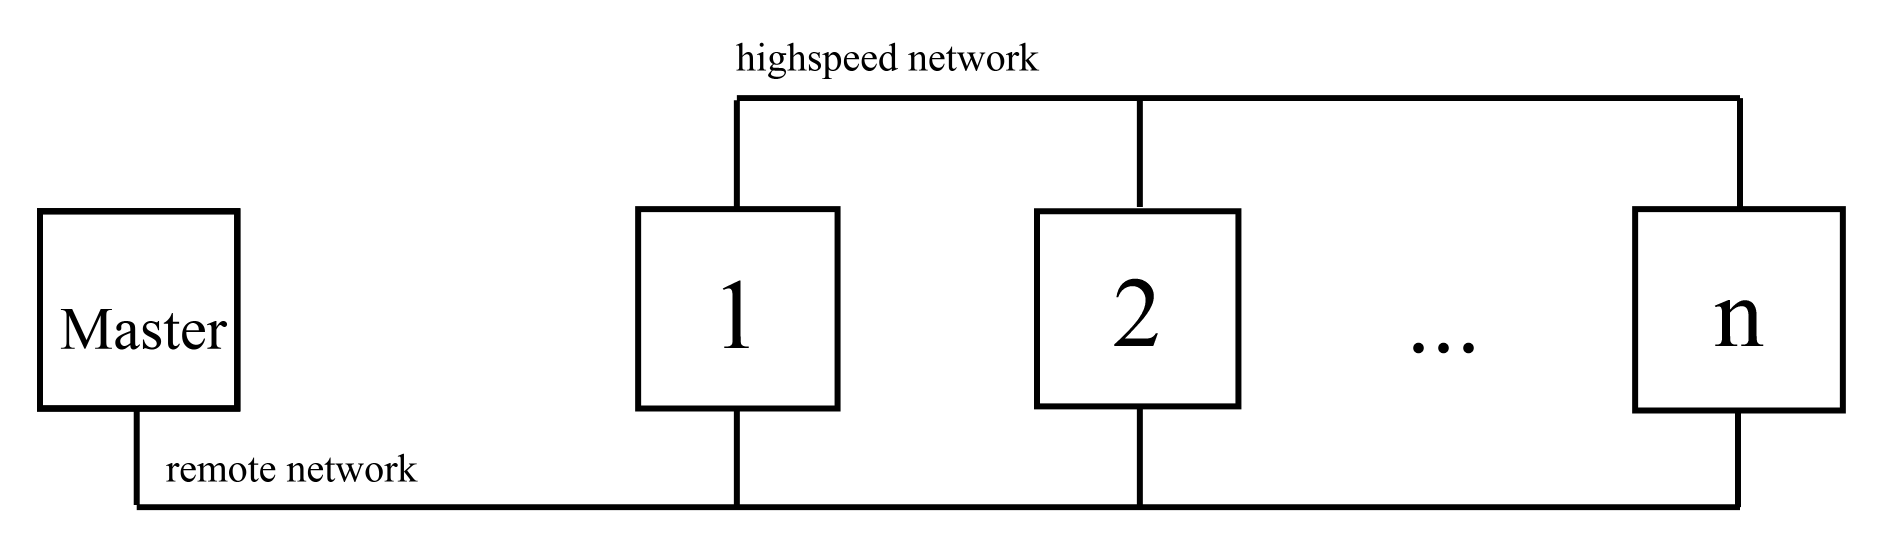
\includegraphics[width=200px]{gfx/cluster_computing.png}
	\caption{cluster computing}
	\label{img:cluster_comp}
\end{figure}
\item grid computing(virtual organisation, geographically distributed and heterogenous))
\end{compactitem}
\item distributed inforamtion systems
\begin{compactitem}
\item transaction processing systems (database) \\
ACID (atomicity, consistency, isolated, durable)
\item enterprise systems
\end{compactitem}
\item Distributed pervasive systems\\
small, wireless, adhoc, no administration\\
home automation, health systems, sensor networks
\end{compactitem}

\textbf{Why do we need distributed systems?}\\
\begin{compactitem}
\item performance
\item distribution inherent
\item reliability
\item incremental growth (scalability)
\item sharing resources
\end{compactitem}

\chapter{Architectures of distributed Systems}

\begin{compactitem}
\item how to split software into components\\
$\Rightarrow$ Softwarearchiticture
\item how to build a system out of the components\\
$\Rightarrow$ Systemarchitecture
\end{compactitem}

Middleware can  help to create distribution transparency\\

Architecturestyles:\\
\begin{compactitem}
\item Layered architecture\\
$\Rightarrow$ network stack, messages or data flow up and down\\
\begin{compactitem}
\item control flow between layers
\item requests down
\item reply up
\end{compactitem}
\item Object-based architectures\\
\begin{compactitem}
\item interaction between components
\item e.g. remote procedure calls
\item can be client-server system
\end{compactitem}
\item data-centered architectures\\
\begin{compactitem}
\item data is key element
\item communication over data, distributed database
\item web-systems mostly data-centric
\end{compactitem}
\item event-based architecture\\
\begin{compactitem}
\item publish-subscribe systems
\begin{figure}[h]
	\centering
	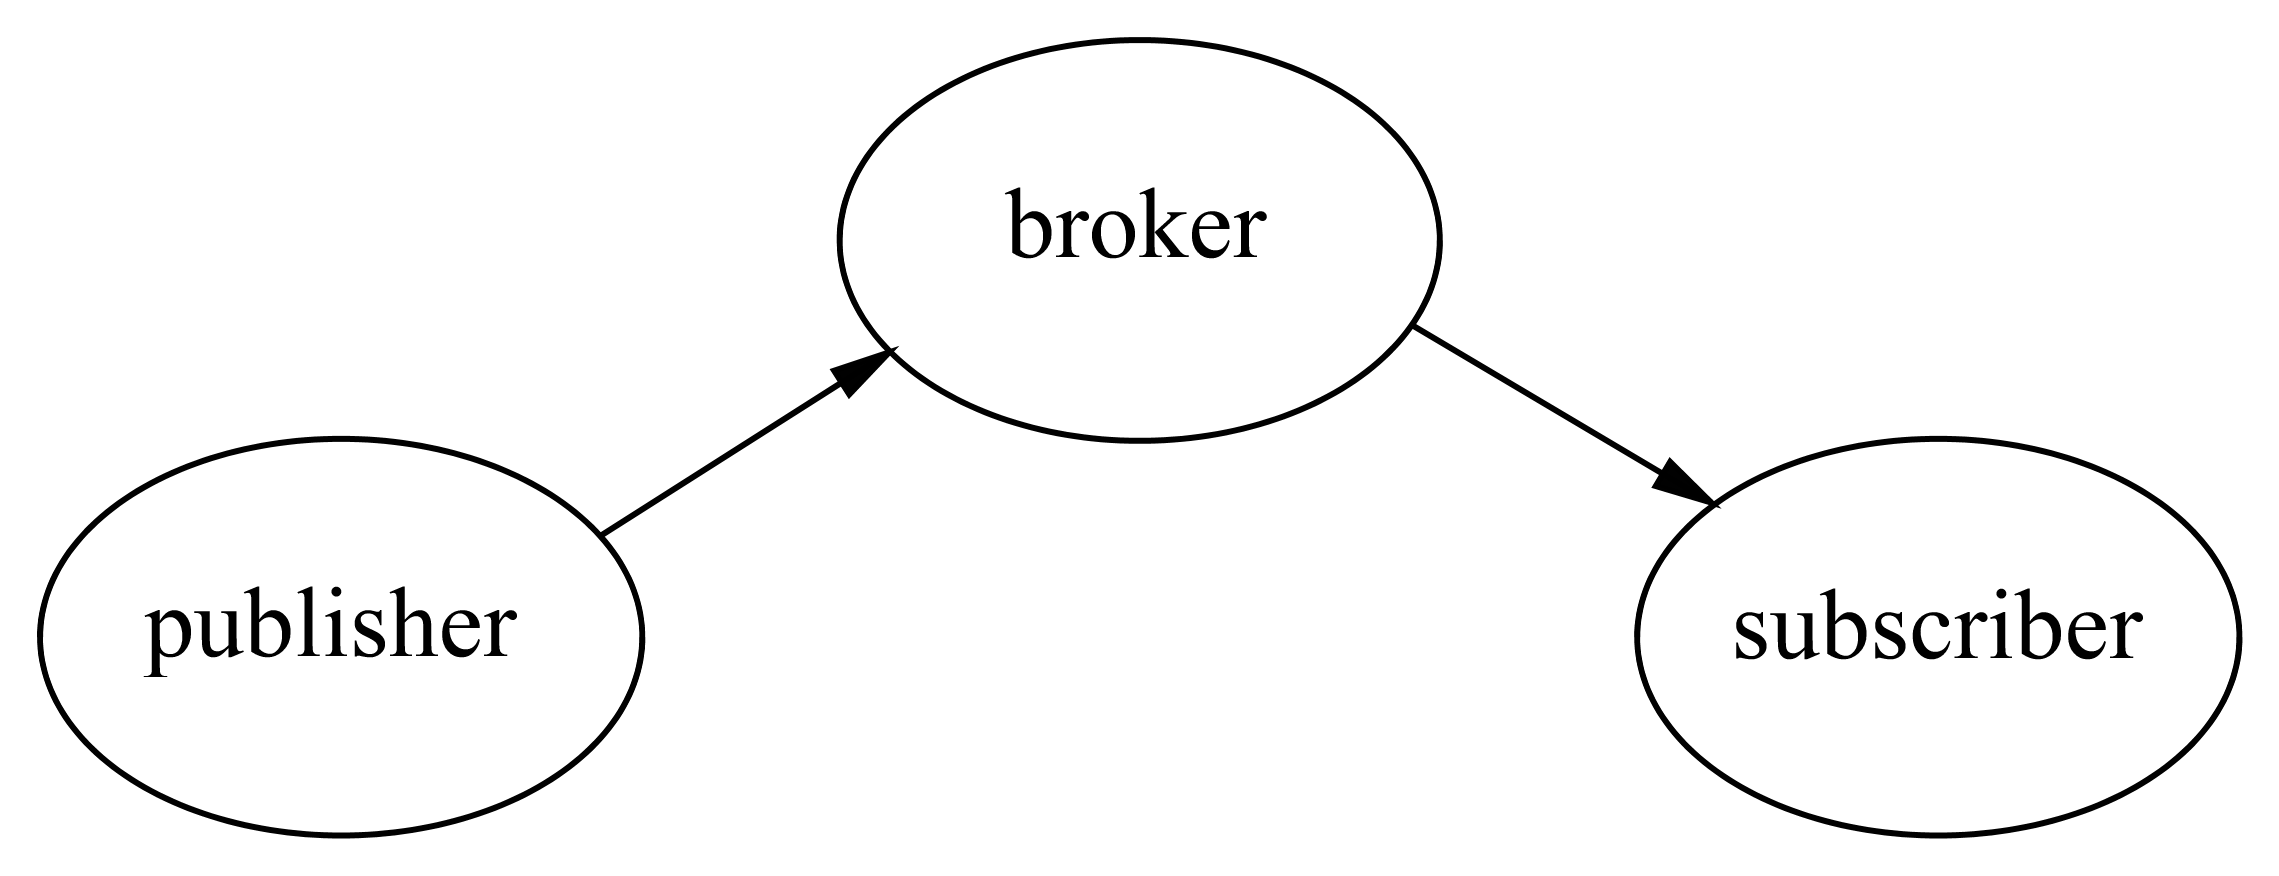
\includegraphics[width=200px]{gfx/pub_sub.png}
	\caption{publish subsribe system}
	\label{img:publish_subscribe}
\end{figure}
\item processes communicates threough events
\item publisher announces events at broker\\
$\Rightarrow$ loose coupling (publisher and subscriber need not to know each other), decoupled in space\\
$\Rightarrow$ scalability better than client-server, parallel processing, caching\\
\end{compactitem}
Event-based and data-based can be combined\\
$\Rightarrow$ shared Data space \\
\begin{figure}[h]
	\centering
	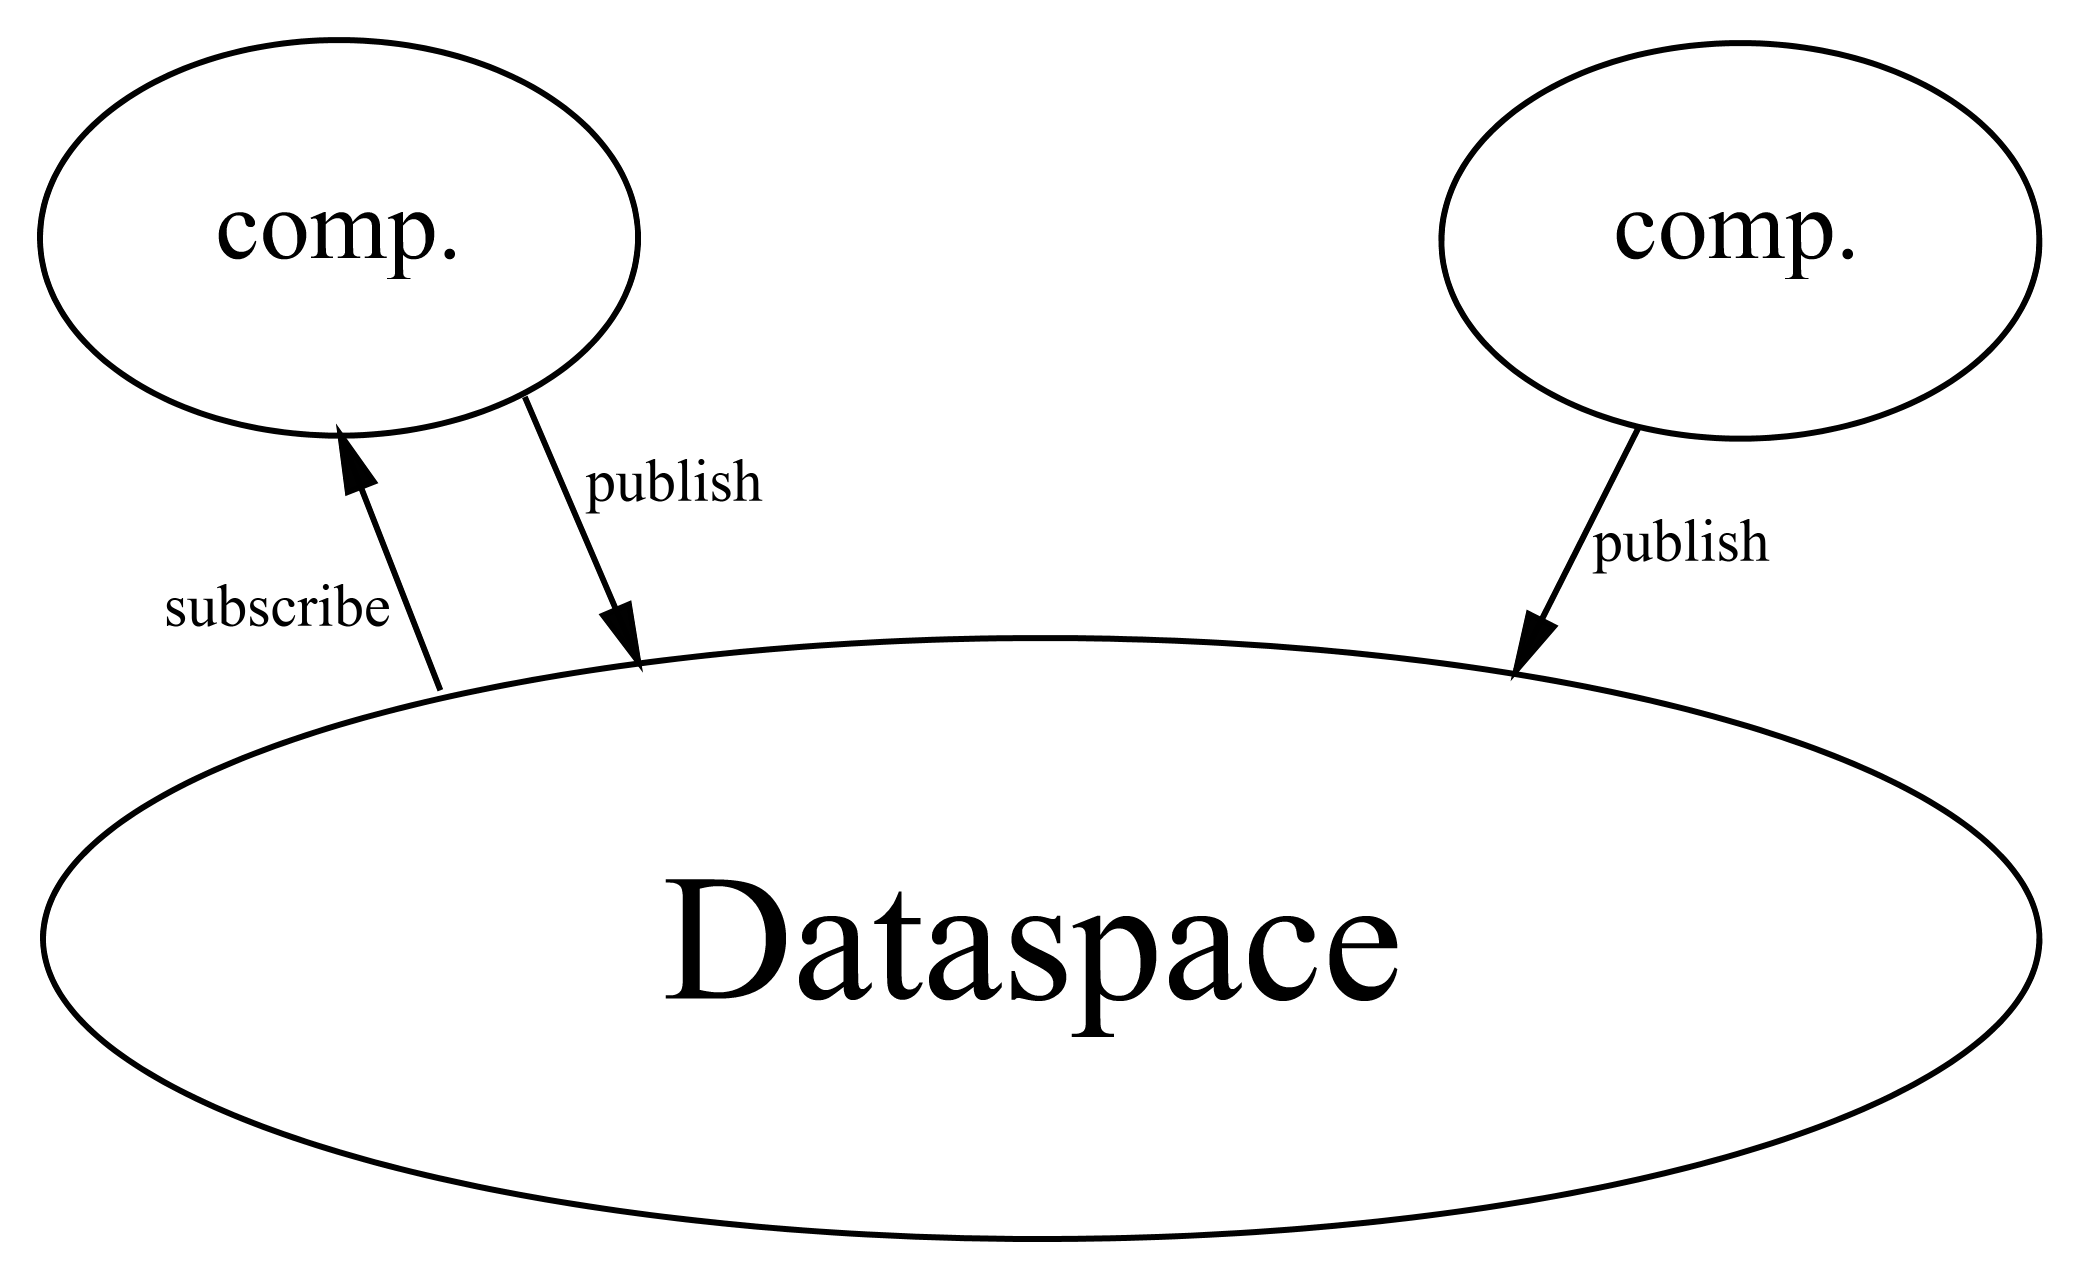
\includegraphics[width=200px]{gfx/shared_data_space.png}
	\caption{shared data space}
	\label{img:shared_data_space}
\end{figure}
\end{compactitem}

\section{System architectures}
\begin{compactenum}
\item centralized architectures\\
client - server\\
\begin{compactitem}
\item[(i)] single point of failure
\item[(ii)] performance (server is bottleneck)\\
\begin{figure}[h]
	\centering
	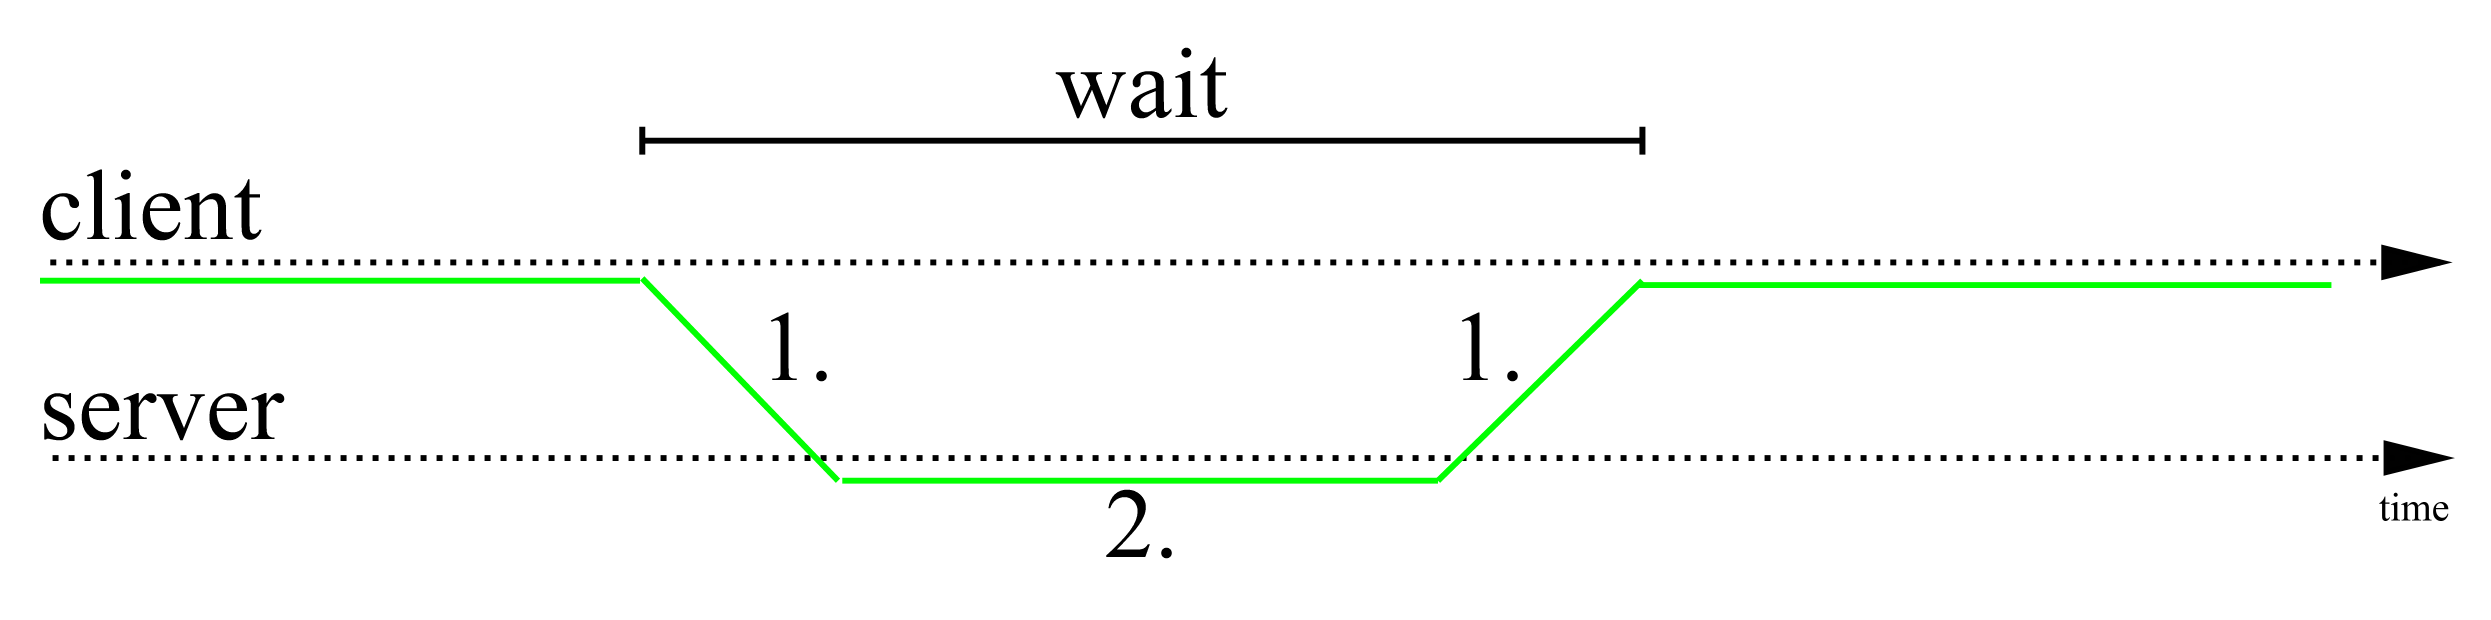
\includegraphics[width=200px]{gfx/cs_simple_wait.png}
	\caption{client server simple waiting situation}
	\label{img:cs_simple_wait}
\end{figure}
\begin{compactenum}
\item communication problems\\
\item server problems\\
\end{compactenum}
can request be repeated without harm?\\
$\Rightarrow$ request is idempotent
\item[(iii)] aplication layering\\
Layers:\begin{compactitem}
\item[1.)] User interface
\item[2.)] processing
\item[3.)] data level
\begin{figure}[h]
	\centering
	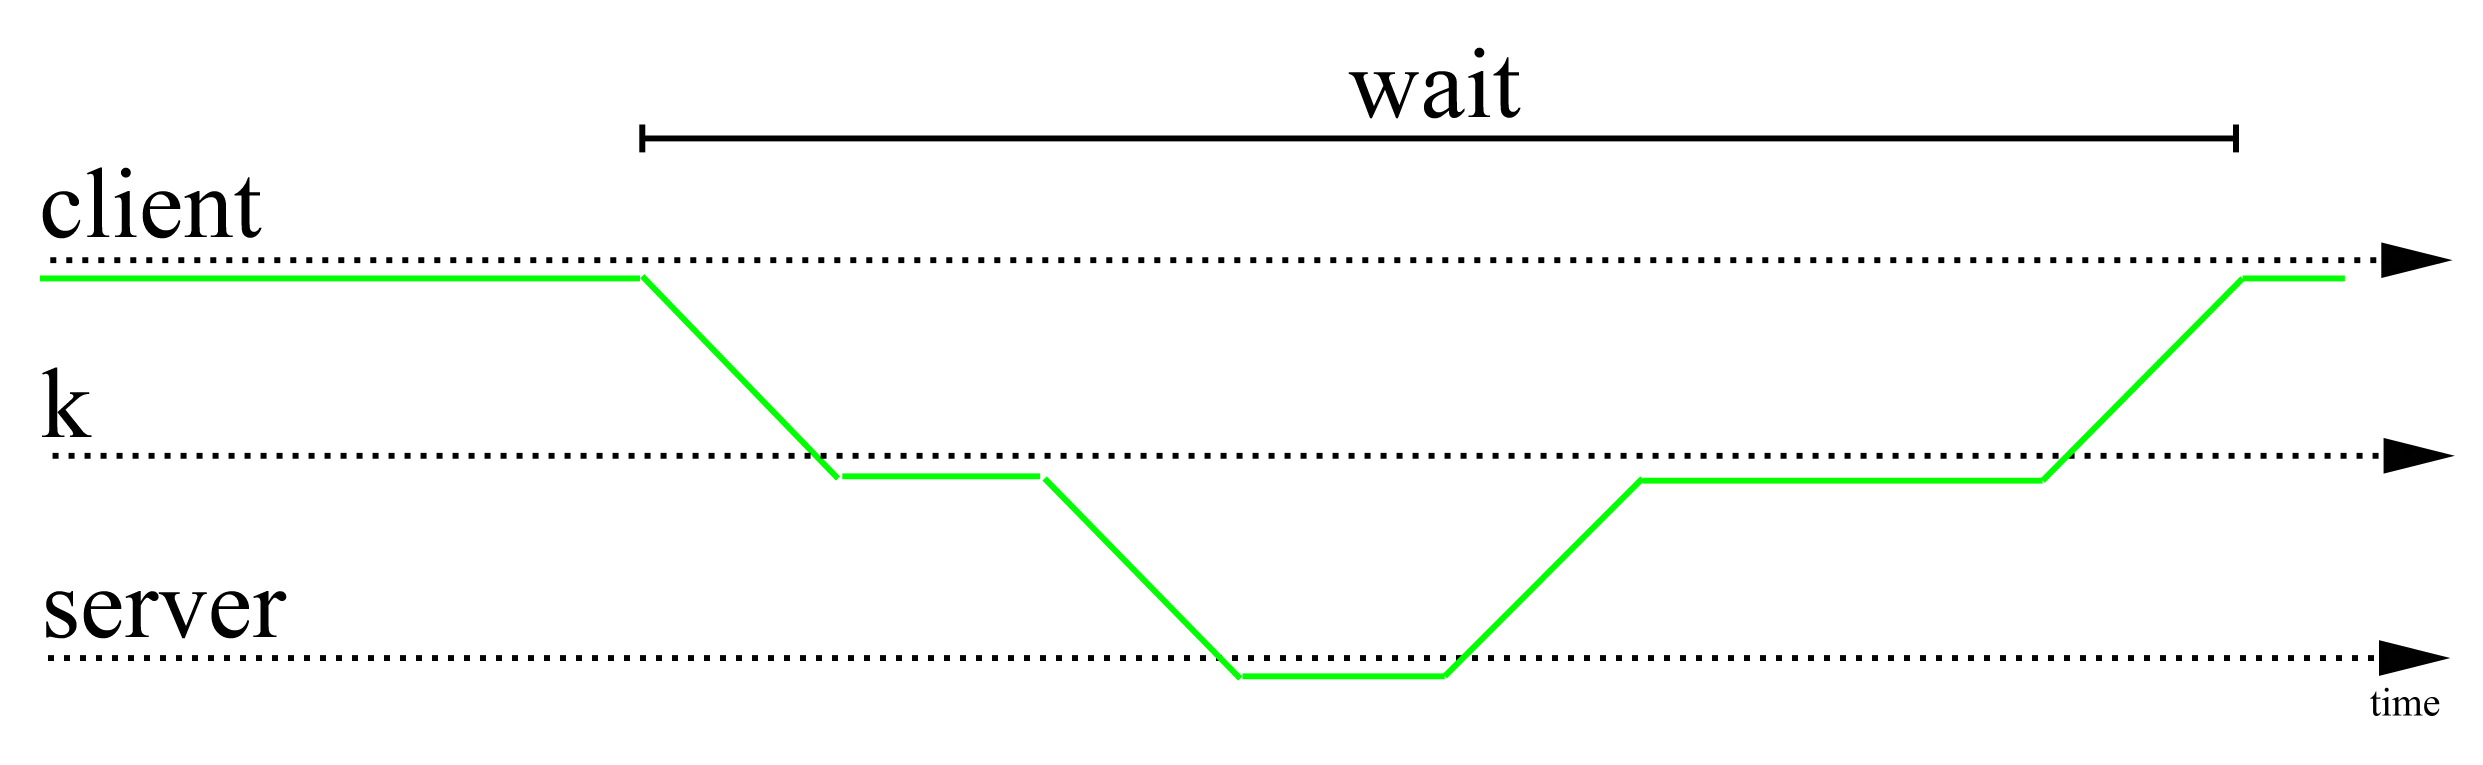
\includegraphics[width=200px]{gfx/cs_app_layer.png}
	\caption{application layer}
	\label{img:cs_app_layer}
\end{figure}
\end{compactitem}
$\Rightarrow$ a lot of waiting\\
$\Rightarrow$ does not scale\\
\end{compactitem}
\item Decentralized architectures\\
\begin{compactitem}
\item vertical distribution (layering)\\
different logic on different machines
\item horizontal distribution \\
replicated client/server operating on different data\\
$\Rightarrow$ overlay-underlay hides physical structure by adding logical structure\\
\end{compactitem}

Structured P2P architectures\\
\begin{compactitem}
\item most popular technique is distributed hashtables (DHT)\\
\item randomly 128 bit or 160 bit ke for data and nodes. Two or more keys are very unlikely\\
\item Chord system arranges items in a ring 
\item data item k is assigened to node with smallest identifier id $\geq$ k
\end{compactitem}
ie item 1 belongs to node 1\\
item 2 belongs to node 2\\
for each item k$_i$ succ(k)=id\\
returns  the name of the node k is assigened to\\
to find data item k the function LOOKUP(k) returns the adress of succ(k) in O(log(N)(later!)\\

membership management\\
join:\\
create SHA1 identifier\\
LOOKUP(id) = succ(id)\\
contact succ(id) and pred(id) to join ring\\

leave:\\
node id informs succ(id) and pred(id) and assigns it's data to succ(id)\\

Content adressable network (CAN)\\
\begin{compactitem}
\item d-dimensional cartesian space
\item every node draws random number
\item space is divided among nodes
\item every data draws identifier (coodinates) which assigns a node

\item join\begin{compactitem}
\item select random point
\item half the square in which id falls
\item assign item to centers
\end{compactitem}
\item leave\begin{compactitem}
\item one node takes the rectangle\\
$\Rightarrow$ reassign rectangles periodically
\end{compactitem}
\end{compactitem}

Unstructured P2P Network\\
\begin{compactitem}
\item random graph
\item each node maintains a list of c neighbours
\item partial view or neighbourhood list  with age
\item nodes exchange neighbour information \\active thread\\ select peer\\

PUSH\\
select c/2 youngest entries+myself\\
send to peer\\

PULL\\
receive peer buffer\\
construct new partial view\\
increment age\\

passive thread\\
recieve buffer from peer\\

PULL:\\
select c/2\\
send to peer\\
construct new partial view
increment age\\

\end{compactitem}

\end{compactenum}


\chapter{PeerSim}

\chapter{Processes}
\begin{tabular}{p{7cm} p{7cm}}
\textbf{processes}			&\textbf{threads}\\
-execution of program			&-several threads share CPU\\
-processor creates virtual processor	&-thread context has little memory information, perhaps mutex lock\\
-for each program everyting is stored in process table	&-threads avoid blocking application (e.g. spreadsheet,computation of dependent cells, intermediate backup)\\
-transparent sharing of resources,(processor, memory) separation&-thread switch is fast\\
-each virtual processor has it's own independent adress space&-user level threads allow parallel computation of program sections\\
-process switch is expensive, (save cpu context, pointers, translation lookaside buffer (TLB), memory management unit (MMU))&I/O or other blocking system calls block all threads, but thread creation/deletion is kernel task = expensive \\
-perhaps even swaps to disk, if memory exhausted& advantages of threads over processes vanishes\\
\end{tabular}

\textbf{Summary:}\\
\begin{compactitem}
\item Serveral threads share one process.
\item Processes have own address space, threads don't.
\item Processes and threads each have userland and kernel implementations
\end{compactitem}

\textbf{2 possible solutions:}\\
\begin{compactenum}
\item scheduler activation, upcall to achieve process switch
\item light-weight processes (LWP)\\
\begin{figure}[h]
	\centering
	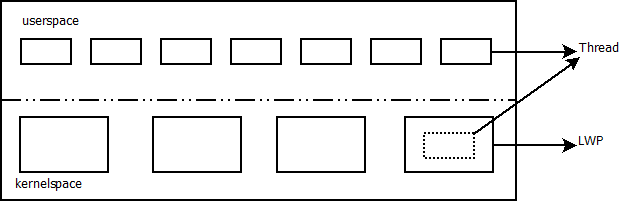
\includegraphics[width=200px]{gfx/thread_lwp.png}
	\caption{light-weight processes can run threads}
	\label{img:lwp_threads}
\end{figure}
user level thread package\\
execute scheduler and run thread of parent\\
may block on systemcall, then other LWP may run\\
triggered from userspace\\
\end{compactenum}
Advantages of LWP and user-level thread package:\\
\begin{compactenum}
\item creation, deletion etc is easy, no kernel intervention
\item blocking syscall does not suspend process if enough LWPs are available
\item applications do not see LWP. They only see user-level threads
\item LWP can run on different processors in multiprocessor systems
\end{compactenum}

Disadvantages:\\
\begin{compactenum}
\item LWP creation as expensive as creation of kernel-level thread
\end{compactenum}

Advantages:\\
- a blocking systemcall blocks only thread, not process
$\Rightarrow$ system call for communication in distributed systems

Multiple threads in clients and servers\\

\textbf{Clients:}\\
\begin{compactitem}
\item multiple thread may hide communication delay (distribution transparency)
\item web browser opens several connections to load parts of a document/page
\item web server may be replicated in same or different location\\
$\Rightarrow$ truly parallel access to items and parallel download
\end{compactitem}

\textbf{Servers:}\\
\begin{compactitem}
\item single threaded, e.g. file server\\
thread serves incoming request, waits for disk, returns file\\
serves next
\item multithreaded\\
dispatcher thread recieves request\\
hands over to worker thread\\
waits for disk etc.\\
dispatcher takes next request
\item finite state machine\\
only one thread\\
examines request, either read from \ldots or from disk\\
during wait stores requests in table\\
serves next request\\
manage control either new request or reply from disk\\
act accordingly\\
process acts as finite state machine that receives messages and acts/changes state
\end{compactitem}


\textbf{Summary:}\\
\begin{tabular}{l l}
model&characteristics\\
single thread& no parallelism, blocking syscalls\\
multi thread& parallelism, blocking syscalls\\
finite state machine& parallelism, non-blocking syscalls\\
\end{tabular}

\section{Virtualisation}
% Bild von Höpster
\begin{figure}[h]
	\centering
	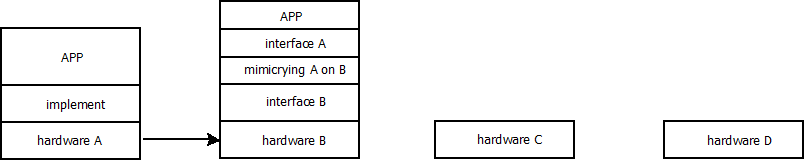
\includegraphics[width=400px]{gfx/virtualisation_1.png}
	\caption{virtualisation}
	\label{img:virtualisation_1}
\end{figure}

V pretends there are more resources then available.\\

Reasons for the need for Virtualization\\
-hardware changes much faster then SW\\
$\Rightarrow$ improves portability\\
-networks consist of different hardware\\
$\Rightarrow$ enables portability of programs for all\\
usage (distributed applications, network protocols)\\

2 Types of Architectures for Virtualisation:\\
\begin{compactenum}
\item Runtime system providing instruction set\\
    Virtualization of processes (e.g. Wine)\\
	\begin{compactitem}
	\item interpreted as Java
	\item emulated as for Windows applications on UNIX-platform processes VM
	\end{compactitem}
\item Virtualisation shields hardware and offers instruction set of the same or other hardware\\
- can host different OS that run simultaneosly\\
$\Rightarrow$ VMM such as VMware, Xen\\


\end{compactenum}


\section{Client-/Serverprocesses}
\textbf{Clients:}\\
%Bild von Tobi !!! :D
\begin{figure}[h]
	\centering
	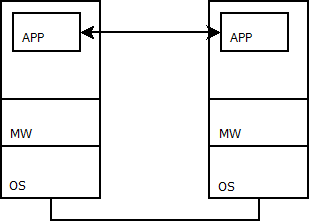
\includegraphics[width=200px]{gfx/clienta.png}
	\caption{app specific communication}
	\label{img:clienta}
\end{figure}
%Mehr Bild!
\begin{figure}[h]
	\centering
	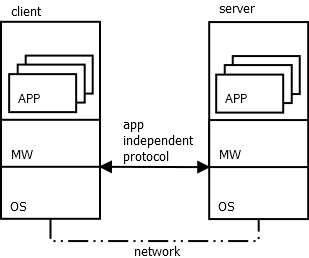
\includegraphics[width=200px]{gfx/clientb.png}
	\caption{machine only communication}
	\label{img:clientb}
\end{figure}

\begin{compactitem}
\item b) allows to store data at the server
\item \textbf{thin client} e.g. X-windows
\item thin client should separate application logic from user interaction
\item often not implemented $\Rightarrow$ poor performance
\item compression of interaction commands as solution
\item compound documents where user interaction triggers several processing steps on the server. must be implemented (e.g. rotation of picture changes placement in texts)
\end{compactitem}

\textbf{Servers:}\\
\begin{compactitem}
\item serves requests on behalf of the client (can server one request at a time)
	\item Types of servers\\
		\begin{compactitem}
			\item \textbf{iterative Server} handles requests itself
			\item \textbf{concurrent server} passes requests to worker, e.g. multithreaded server
		\end{compactitem}
	\item server listens to port, endpoint to the client; some ports are reserved for special services
\begin{figure}[h]
	\centering
	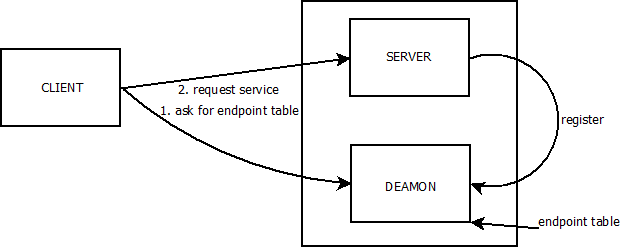
\includegraphics[width=200px]{gfx/server_deamon.png}
	\caption{listener server}
	\label{img:listener}
\end{figure}
	\item superserver listens to several ports, replacinf several (mostly idle) servers
\begin{figure}[h]
	\centering
	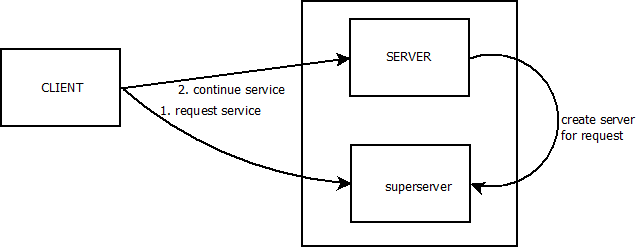
\includegraphics[width=200px]{gfx/superserver.png}
	\caption{superserver}
	\label{img:supserv}
\end{figure}
	\item stateless servers, keeps no information on state of client $\rightarrow$ change state without informing the client, e.g. web server
\begin{figure}[h]
	\centering
	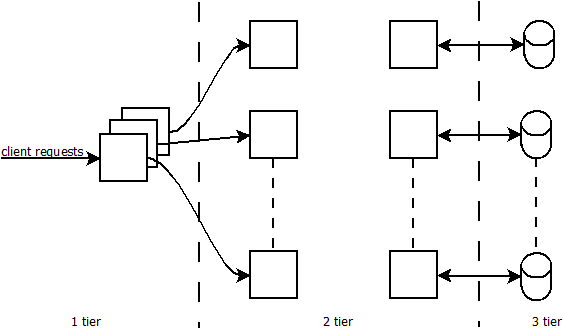
\includegraphics[width=200px]{gfx/server3.png}
	\caption{stateless server}
	\label{img:statel_serv}
\end{figure}
	\item soft state server, maintains client state for limited time, e.g. servers informing about updates
	\item stateful server keeps information about client (file server keeps (client, file) table), often better performance, fault-tolerance poorer
	\item cookies allow to share information for server upon next visit client sends it'S cookies, allows state information for stateless server

\end{compactitem}
\textbf{Distributed Servers}\\
\begin{figure}[h]
	\centering
	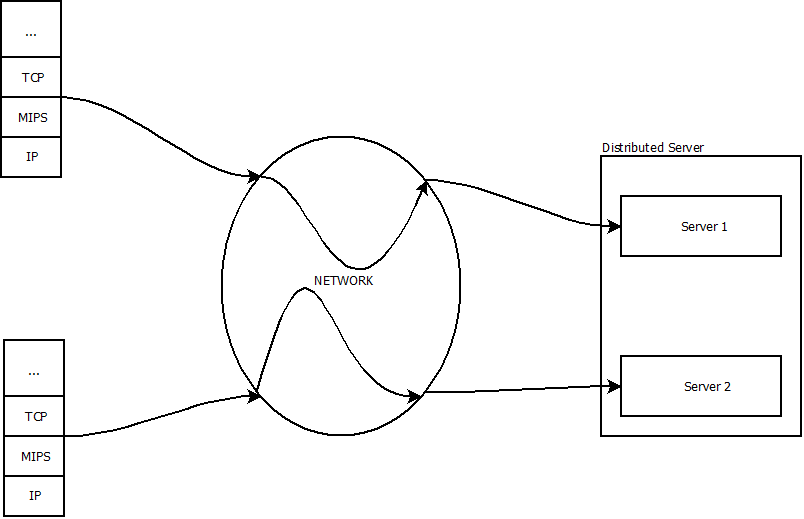
\includegraphics[width=200px]{gfx/distrb_server.png}
	\caption{distributed server}
	\label{img:distrb_serv}
\end{figure}
\begin{compactitem}
	\item servers in different locations that have different ip-adresses in DNS under the same name
	\item MIPv6: mobility support for IPv6
	\item mobile node has home network with stable home adress (HoA)
	\item special router is home agent and takes care of traffic to the mobile node
	\item mobile node receives care-of-adress (CoA), never seen by client
	\item route optimisation avoids routing through home agent
\end{compactitem}

\section{Code Migration}
\begin{compactitem}
	\item Code migration on (running) process - Why?
	\item service placement in distributed system $\Rightarrow$ minimize communication cost
	\item load balancing in multiprocessor machine or cluster $\Rightarrow$ performace
	\item (security)

\end{compactitem}

\textbf{Models of Migration}
\begin{compactitem}
	\item or process model\begin{compactenum}
		\item code segment, instructions
		\item resource segement, references to external resources, ie.e. file, printer, devices
		\item execution segement, execution state process, stack, private data, programm counter

	\end{compactenum}
	\item \textbf{Migration types}\begin{compactitem}
		\item weak mobility, transfer code, (1), mabe 3)), which executes from beginning (i.e. java applets)
		\item strong mobility, transfer 1)3), stop executions, transfer, resume
	\end{compactitem}
\end{compactitem}

%bild

Migrating resource segment 2) is difficult\\
Consider process to resource binding\\
\begin{compactenum}
	\item binding by identifier, URL, ftp-server-name
	\item binding by value, libraries for programming
	\item binding by type, local device, monitor
\end{compactenum}

\textbf{Resource-machine-binding}
\begin{compactenum}
	\item unattached
	\item fastend
	\item fixed
\end{compactenum}

\begin{tabular}{l| l| l| l}
pass tp resource binding&unattached&fastened&fixed\\
\hline
by identifier& MV&GR(or MV)& GR\\
\hline
by value& CP& GR(or CP)& GR\\
\hline
by type& RB&RB(or GR,CP)&RB(or GR)\\
\end{tabular}
MV:move, GR, global reference, CP: copy value, RB: rebind to locally available resource


%\chapter{Processes}
%\begin{tabular}{p{7cm} p{7cm}}
%\textbf{processes}			&\textbf{threads}\\
%-execution of program			&-several threads share CPU\\
%-processor creates virtual processor	&-thread context has little memory information, perhaps mutex lock\\
%-for each program everyting is stored in process table	&-threads avoid blocking application (e.g. spreadsheet,computation of dependent cells, intermediate backup)\\
%-transparent sharing of resources,(processor, memory) separation&-thread switch is fast\\
%-each virtual processor has it's own independent adress space&-user level threads allow parallel computation of program sections\\
%-process switch is expensive, (save cpu context, pointers, translation lookaside buffer (TLB), memory management unit (MMU))&I/O or other blocking system calls block all threads, but thread creation/deletion is kernel task = expensive \\
%-perhaps even swaps to disk, if memory exhausted& advantages of threads over processes vanishes\\
%\end{tabular}
%
%2 possible solutions:\\
%\begin{compactenum}
%\item scheduler activation, upcall to achieve process switch
%\item light-weight processes (LWP)\\
%\begin{figure}[h]
%	\centering
%	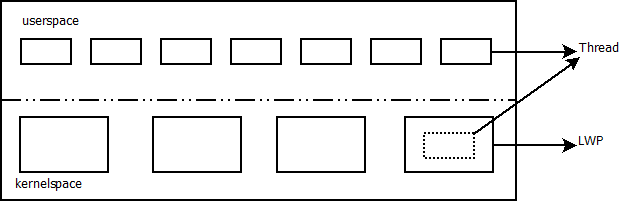
\includegraphics[width=200px]{gfx/thread_lwp.png}
%	\caption{light-weight processes can run threads}
%	\label{img:lwp_threads}
%\end{figure}
%user level thread package\\
%execute scheduler and run thread of parent\\
%may block on systemcall, then other LWP may run\\
%triggered from userspace\\
%\end{compactenum}
%Advantages of LWP and user-level thread package:\\
%\begin{compactenum}
%\item creation, deletion etc is easy, no kernel intervention
%\item blocking syscall does not suspend process if enough LWPs are available
%\item applications do not see LWP. They only see user-level threads
%\item LWP can run on different processors in multiprocessor systems
%\end{compactenum}
%
%Disadvantages:\\
%\begin{compactenum}
%\item LWP creation as expensive as creation of kernel-level thread
%\end{compactenum}
%
%Advantages:\\
%- a blocking systemcall blocks only thread, not process
%$\Rightarrow$ system call for communication in distributed systems
%
%Multiple threads in clients and servers\\
%
%\textbf{Clients:}\\
%\begin{compactitem}
%\item multiple thread may hide communication delay (distribution transparency)
%\item web browser opens several connections to load parts of a document/page
%\item web server may be replicated in same or different location\\
%$\Rightarrow$ truly parallel access to items and parallel download
%\end{compactitem}
%
%\textbf{Servers:}\\
%\begin{compactitem}
%\item single threaded, e.g. file server\\
%thread serves incoming request, waits for disk, returns file\\
%serves next
%\item multithreaded\\
%dispatcher thread recieves request\\
%hands over to worker thread\\
%waits for disk etc.\\
%dispatcher takes next request
%\item finite state machine\\
%only one thread\\
%examines request, either read from \ldots or from disk\\
%during wait stores requests in table\\
%serves next request\\
%manage control either new request or reply from disk\\
%act accordingly\\
%process acts as finite state machine that receives messages and acts/changes state
%\end{compactitem}
%
%\textbf{summary:}\\
%\begin{tabular}{l l}
%model&characteristics\\
%single thread& no parallelism, blocking syscalls\\
%multi thread& parallelism, blocking syscalls\\
%finite state machine& parallelism, non-blocking syscalls\\
%\end{tabular}
%
%\section{Virtualisation}
%% Bild von Höpster
%\begin{figure}[h]
%	\centering
%	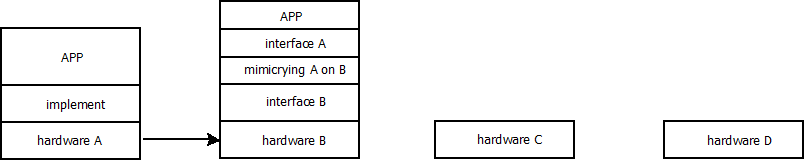
\includegraphics[width=200px]{gfx/virtualisation_1.png}
%	\caption{virtualisation}
%	\label{img:virtualisation_1}
%\end{figure}
%
%V pretends there are more resources then available.\\
%
%Reasons for the need for V.\\
%-hardware changes much faster then SW\\
%$\Rightarrow$ improves portability\\
%-networks consist of different hardware\\
%$\Rightarrow$ enables portability of programs for all\\
%usage (distributed applications, network protocols)\\
%
%2 Types of Architectures for Virtualisation:\\
%\begin{compactenum}
%\item Runtime system providing instruction set\\
%	\begin{compactitem}
%	\item interpreted as Java
%	\item emulated as for Windows applications on UNIX-platform processes VM
%	\end{compactitem}
%\item Virtualisation shields hardware and offers instruction set of the same or other hardware\\
%- can host different OS that run simultaneosly\\
%$\Rightarrow$ VMM such as VMware, Xen\\
%
%
%\end{compactenum}
%
%
%\section{Client-/Serverprocesses}
%\textbf{CLients:}\\
%%Bild von Tobi !!! :D
%\begin{figure}[h]
%	\centering
%	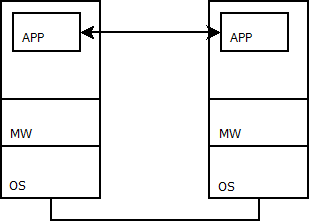
\includegraphics[width=200px]{gfx/clienta.png}
%	\caption{app specific communication}
%	\label{img:clienta}
%\end{figure}
%%Mehr Bild!
%\begin{figure}[h]
%	\centering
%	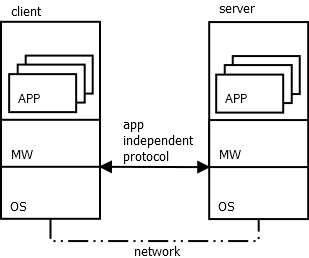
\includegraphics[width=200px]{gfx/clientb.png}
%	\caption{machine only communication}
%	\label{img:clientb}
%\end{figure}
%
%\begin{compactitem}
%\item b) allows to store data at the server
%\item \textbf{thin client} e.g. X-windows
%\item thin client should separate application logic from user interaction
%\item ooften not implemented $\Rightarrow$ poor performance
%\item compression of interaction commands as solution
%\item compound documents where user interaction triggers several processing steps on the server. must be implemented (e.g. rotation of picture changes placement in texts)
%\end{compactitem}
%
%\textbf{Servers:}\\
%\begin{compactitem}
%	\item serves requests on behalf of the client
%	\item Types of servers\\
%		\begin{compactitem}
%			\item \textbf{iterative Server} handles requests itself
%			\item \textbf{concurrent server} passes requests to worker, e.g. multithreaded server
%		\end{compactitem}
%	\item server listens to port, endpoint to the client; some ports are reserved for special services
%\begin{figure}[h]
%	\centering
%	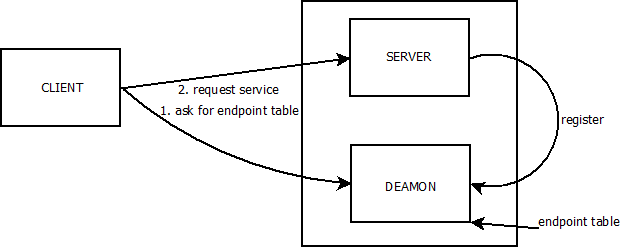
\includegraphics[width=200px]{gfx/server_deamon.png}
%	\caption{listener server}
%	\label{img:listener}
%\end{figure}
%	\item superserver listens to several ports, replacinf several (mostly idle) servers
%\begin{figure}[h]
%	\centering
%	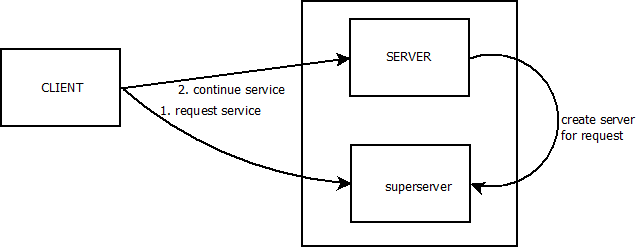
\includegraphics[width=200px]{gfx/superserver.png}
%	\caption{superserver}
%	\label{img:supserv}
%\end{figure}
%	\item stateless servers, keeps no information on state of client $\rightarrow$ change state without informing the client, e.g. web server
%\begin{figure}[h]
%	\centering
%	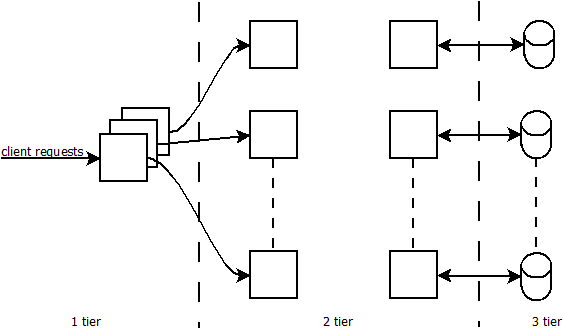
\includegraphics[width=200px]{gfx/server3.png}
%	\caption{stateless server}
%	\label{img:statel_serv}
%\end{figure}
%	\item soft state server, maintains client state for limited time, e.g. servers informing about updates
%	\item stateful server keeps information about client (file server keeps (client, file) table), often better performance, fault-tolerance poorer
%	\item cookies allow to share information for server upon next visit client sends it'S cookies, allows state information for stateless server
%
%\end{compactitem}
%\textbf{Distributed Servers}\\
%\begin{figure}[h]
%	\centering
%	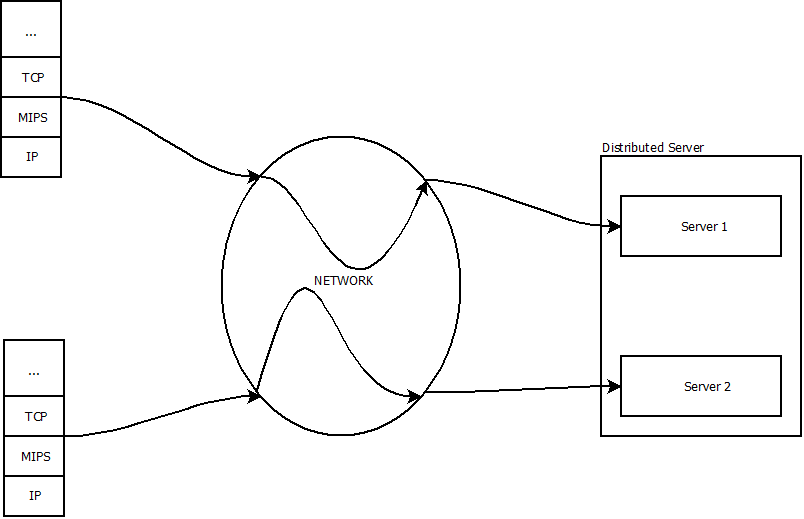
\includegraphics[width=200px]{gfx/distrb_server.png}
%	\caption{distributed server}
%	\label{img:distrb_serv}
%\end{figure}
%\begin{compactitem}
%	\item servers in different locations that have different ip-adresses in DNS under the same name
%	\item MIPv6: mobility support for IPv6
%	\item mobile node has home network with stable home adress (HoA)
%	\item special router is home agent and takes care of traffic to the mobile node
%	\item mobile node receives care-of-adress (CoA), never seen by client
%	\item route optimisation avoids routing through home agent
%\end{compactitem}
%
%\section{Code Migration}
%\begin{compactitem}
%	\item Code migration on (running) process - Why?
%	\item service placement in distributed system $\Rightarrow$ minimize communication cost
%	\item load balancing in multiprocessor machine or cluster $\Rightarrow$ performace
%	\item (security)
%
%\end{compactitem}
%
%\textbf{Models of Migration}
%\begin{compactitem}
%	\item or process model\begin{compactenum}
%		\item code segment, instructions
%		\item resource segement, references to external resources, ie.e. file, printer, devices
%		\item execution segement, execution state process, stack, private data, programm counter
%
%	\end{compactenum}
%	\item \textbf{Migration types}\begin{compactitem}
%		\item weak mobility, transfer code, (1), mabe 3)), which executes from beginning (i.e. java applets)
%		\item strong mobility, transfer 1)3), stop executions, transfer, resume
%	\end{compactitem}
%\end{compactitem}
%
%%bild
%
%Migrating resource segment 2) is difficult\\
%Consider process to resource binding\\
%\begin{compactenum}
%	\item binding by identifier, URL, ftp-server-name
%	\item binding by value, libraries for programming
%	\item binding by type, local device, monitor
%\end{compactenum}
%
%\textbf{Resource-machine-binding}
%\begin{compactenum}
%	\item unattached
%	\item fastend
%	\item fixed
%\end{compactenum}
%
%\begin{tabular}{l| l| l| l}
%pass tp resource binding&unattached&fastened&fixed\\
%\hline
%by identifier& MV&GR(or MV)& GR\\
%\hline
%by value& CP& GR(or CP)& GR\\
%\hline
%by type& RB&RB(or GR,CP)&RB(or GR)\\
%\end{tabular}
%MV:move, GR, global reference, CP: copy value, RB: rebind to locally available resource
%
\chapter{Communication}

\begin{compactitem}
	\item Communication in distributed systems is always based on low-level message passing as offered by the underlying network
	\item message passing is harder than using primitives based on shared memory, as in nondistributed systems
	\item low-level communication facilities of computer networks are in many ways not suitable due to their lack of distribution transparency.
\end{compactitem}

\section{RPC - Remote Procedure Call}
%ordinary procedure call, e.g. count = read(fd,buf,nbytes)

\begin{compactitem}
	\item allow programs to call procedures located on other machines
	\item When a process on machine A calls' a procedure on machine B, the calling process on A is suspended, and execution of the called procedure takes place on B.
	\item Remote procedure call uses stubs to pack parameters in message
	\item client stub: packs the parameters into a message and requests that message to be sent to the server
	\item server stub: transforms requests coming in over the network into local procedure calls
	\item No message passing at all is visible to the programmer
	\item neither client nor server need to be aware of the intermediate steps or the existence of the network
\end{compactitem}

\subsection*{A remote procedure call occurs in the following steps:}

\begin{enumerate}
	\item The client procedure calls the client stub in the normal way. 
	\item The client stub builds a message and calls the local operating system. 
	\item The client's as sends the message to the remote as. 
	\item The remote as gives the message to the server stub. 
	\item The server stub unpacks the parameters and calls the server.
	\item The server does the work and returns the result to the stub. 
	\item The server stub packs it in a message and calls its local as. 
	\item The server's as sends the message to the client's as. 
	\item The client's as gives the message to the client stub. 
	\item The stub unpacks the result and returns to the client.
\end{enumerate}

\subsection*{Parameter Marshaling}

parameter marshaling: packing parameters into a message is called 


\subsubsection*{Passing Value Parameters}

\begin{compactitem}
	\item values are packed into messages (client) and unpacked from messages (server)
	\item transfered byte-by-byte
	\item as long as the client and server machines are identical this model works fine
	\item in a large distributed system, it is common that multiple machine types are present
	\item $\Rightarrow$ problems because of different character encoding (EBCDIC vs ASCII), represetation of integers (one's complement vs two's complement) or endianness (little endian vs. big endian)
\end{compactitem}

\subsubsection*{Passing Reference Parameters}
\begin{compactitem}
	\item extremly difficult
	\item pointers are meaningful only within the address space of the process in which it is being used
	\item replace with copy/restore: copy the datastructure, send it to the server, work on it, send it back, restore at the client
\end{compactitem}



\section{Asynchronous RPC}

\begin{figure}[h]
	\centering
	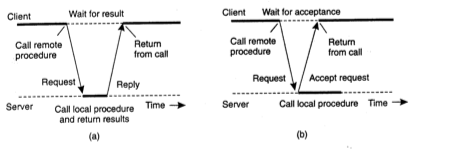
\includegraphics[width=400px]{gfx/rpc.png}
	\caption{a: synchronous b: asynchronous RPC}
	\label{img:rpc}
\end{figure}

\begin{compactitem}
	\item in conventional procedure calls, when a client calls a remote procedure, the client will block until a reply is returned
	\item asynchronous RPCs: the server immediately sends a reply back to the client the moment the RPC request is received. Reply acts as an acknowledgment.
	\item client will continue without further blocking as soon as it has received the server's acknowledgment
	\item Examples: transferring money from one account to another, adding entries into a database, starting remote services, batch processing...
	\item Asynchronous RPCs can also be useful when a reply will be returned but the client doesn't need to wait for it and can do nothing in the meantime
	\item One-Way RPCs: the client does not wait for an acknowledgment from the server
	\item deferred synchronous RPC: organize the communication between the client and server through two asynchronous RPCs
\end{compactitem}

\begin{compactitem}
	\item foo
\end{compactitem}

\section{Message oriented communication}

General Idea: avoid synchronous communication which blocks sender (RPC)

\subsection{Message-Oriented Transient Communication}

transient: flüchtig, vorrübergehend

\subsubsection{Berkeley Sockets}

A socket is a communication end point to which an application can write data that are to be sent out over the underlying network, and from which incoming data can be read. A socket forms an abstraction over the actual communication end point that is used by the local operating system for a specific transport protocol.

\begin{figure}[h]
	\centering
	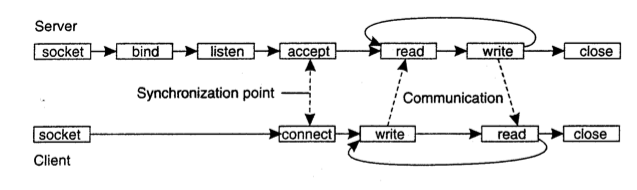
\includegraphics[width=400px]{gfx/sockets.png}
	\caption{Connection-oriented communication pattern using sockets}
	\label{img:sockets}
\end{figure}

\begin{compactitem}
	\item socket: create a new communication end point
	\item bind: attach a local addres to a socket
	\item listen: announce willingness to accept connections
	\item accept: block caller until a connection request arrives
	\item connect: actively attemt to establish a connection
	\item send: send some data over the connection
	\item receive: receive some data over the connection
	\item close: release the connection
\end{compactitem}

\subsubsection{Message-passing-interface (MPI)}
\begin{compactitem}
	\item standad for message passing
	\item designed for parallel applications
	\item communication within groups of processes
	\item A $(groupID, processID)$ pair uniquely identifies the source or destination of a message (used instead of a transport-level address)
\end{compactitem}

\subsection{Message-Oriented Persistent Communication}

aka Message-queuing-system, Message-oriented-middleware (MoM) \\

\begin{figure}[h]
	\centering
	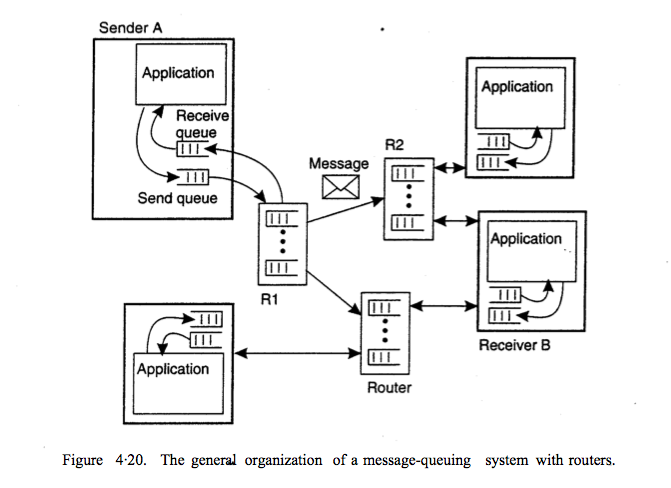
\includegraphics[width=400px]{gfx/mom.png}
	\caption{general organization of a message-queuing system with routers}
	\label{img:mom}
\end{figure}

\begin{compactitem}
	\item asynchronous persistent communication
	\item offer intermediate-term storage capacity for messages, without requiring either the sender or receiver to be active during message transmission
	\item transfer may take minutes, not milliseconds
	\item applications communicate by inserting messages into queues
	\item messages are only put into and read from local queues
	\item the message-queuing system takes care that messages are transferred from their source to their destination queue	
	\item message carries destination address
	\item queue managers
	\begin{compactitem}
		\item a queue manager interacts directly with the application that is sending or receiving a message
		\item also special queue managers that operate as routers, or relays: they forward incoming messages to other queue managers
	\end{compactitem}
	\item message brokers transform type A into type B, using a set of rules
		\begin{compactitem}
		\item application-level gateway in a message-queuing system
		\item convert incoming messages so that they can be understood by the destination application		
		\item transform messages of type A into type B, using a set of rules
	\end{compactitem}
	\item Examples: Email, workflow, batch processing, queries accross several databases
\end{compactitem}

\section{stream oriented communication}
\begin{compactitem}
	\item temporal relationship between items important
	\item multimedia data is compressed
	\item QoS is important\\
		\begin{compactitem}
			\item bit rate
			\item max delay for session setup
			\item max end-to-end delay
			\item max delay variance (jitter)
			\item max round trip delay\\
				% next pic, tobi
		\end{compactitem}
	\item networking solution such as differentiated services
	\item synchronisation of streams
\end{compactitem}
\section{Multicast communication}
\begin{compactitem}
	\item application level multicast uses overlay
	\item tree, unique path between each pair of nodes
	\item mesh, more robust, fault-tolerant
\end{compactitem}
\textbf{Example:} Construct overlay tree for chord
\begin{compactitem}
	\item node that wants to start multicast generates key 128bit/160bit (nid) randomly
	\item lookup of succ(nid) finds node responsible for key mid\\
		$\Rightarrow$ succ(nid) becomes root of tree
	\item join: lookup (nid) creates lookup message with join request routed from P to succ(nid)
	\item request is forwarded Q (first time forward), Q becomes forwarder\\
		$\Rightarrow$ P child of Q
	\item request is first time forwarded by R, R becomes forwarder\\
		$\Rightarrow$ Q becomes child of R
	\item multicast: lookup(nid) sends message to the root\\
		multicast from root
\end{compactitem}
\textbf{Efficiency?}\\
Quality of application level tree\\
\begin{compactenum}
	\item Link stress, number of traversals of same link per packet
	\item stretch, relative delay penalty (RDP)\\
		$\frac{\text{transmission time in overlay}}{\text{transmission time in delay/network}}$
		$\Rightarrow$ minimize aggregated stretch, average RDP over all note pairs
	\item tree cost, minimize aggregated link cost, link cost = cost between end points\\
		$\Rightarrow$ find minimal spanning tree
\end{compactenum}
\section{Gossip-based-communication}
\begin{compactitem}
	\item epidemic behaviour
	\item a node does not have new data (susceptible), it has the data (infected) or is unwilling to spread (removed)\\
	Anti-entropy-model\\
	P chooses randomly Q\\
	\begin{compactenum}
		\item P pushes its data to Q
		\item P pulls Q's data
		\item P and Q exchange data
	\end{compactenum}
	\item if many nodes are infected probabiltry for selecting susceptible node  is low\\
	$\Rightarrow$ low probability of data dissemination\\
	\item pull works when many nodes are infected. Susceptible node determines spread. They have a high probability to contact infected nodes
	\item if only one node is infected push/pull is best
	\item Round is period in which each node at least once selects a neighbor\\
		number of rounds needed to spread  $\approx \mathcal{O}(\log(N)), N$ is number of nodes\\
\end{compactitem}
\textbf{Rumor spreading, gossiping}:\\
%bild
function of nodes that never obtain data: $s=e^{-(k+1)(1-s)}$\\
e.g. $k=4, ln(s) = 4,97$\\
$\Rightarrow s = 0,007$\\
less than $0,7$ remain without data\\
removing data is difficult : delete message is send via gossiping

\chapter{Naming}
Flat naming\\
\section{Distributed Hash Tables}
%krasse büld von de hipster tobi
\begin{compactitem}
\item m-bit identifier (128 or 160 Bit)
\item entity with key k is under jurisdiction of node with smallest identifier id $\geq$ k\\
$\Rightarrow$ succ(k)
\item resolve key k to address of succ(k)
\item option 1: each node p keeps succ(p), pred(p) node forwards request for key k to a neighbor\\
if pred(p) < k $\leq$ p, return(p)\\
$\Rightarrow$ not scalable
\item better solution: each Chord node maintains
\underline{finger table} of lenght m\\

$ \forall \  1 \leq k \leq m :	FT[i] = succ(n+2^{k+1}) \mod 2^m $


\\
FT[$i$]=succ($p+2^{i-1}$) = succ($p+1$) = succ($2$) (smallest id, sucht that id $\geq$ 2)\\
i-th entry points to $2^{i-1}$ ahead of p
\item to lookup k node p forwards request to p with index j in ps finger table:\\
$q = FT_p[j] \leq k \leq FT_p[j+1]$
\item example:\\
resolve k = 26 from node 1 \\
$k=26 > FT_1[5] \Rightarrow$ forward request to node\\
$18 = FT_1[5]$
\begin{compactitem}
\item node $18$ selects node $20 FT_{18}[2] \leq k < FT_{18}[3]$\\
\item node $20$ selects node $21 \Rightarrow 28 $ which is responsible for key $26$\\
\item lookup generally requires $O(log(N))$ steps, N nodes in system
\item join/leave is rather simple
\item keeeping figer table up to date is expensive
\end{compactitem} 
\end{compactitem}


\chapter{Synchronistation}
\section{Clock synchronisation algorithms}
System model: each machine has timer that causes H interrupts per second
\begin{compactitem}
	\item clock $C$ adds up ticks (interrupts)
	\item $C_p(t)$ is clock time on machine $p$
	\item perfect clock: $C_p(t) = t \forall p, t$ \\
	$\Longleftrightarrow C_p'(t) = \frac{d C_p(t)}{dt} = 1$\\
	$\mathrel{\widehat{=}}$ frequency of clock $C_p$ at time $t$
% diagramm vom hipster
	\item $C_p'(t) - 1 \mathrel{\widehat{=}}$ skew of p's clock, difference to perfect clock.
	\item $C_p(t)-t \mathrel{\widehat{=}}$ offset
	\item real timers do not interrupt H timespers maximum drift p such\\
	$1-\rho \leq \frac {d(H)}{dt} \leq 1+p$
	\item at time $\delta t$ two clocks that are drifting apart can be\\
	$|C_2(\Delta t) - C_1(\Delta t) \leq 2 \rho \Delta t|$
	\item if the difference should never exceed $\delta_i$ then synchronisation every $\frac {\delta}{2 \rho}$ seconds is needed
	\item time allways moves forward.
\end{compactitem}


\section{Network Time Protcol (NTP)}
\begin{compactitem}
\item nodes contact time server that has an accurate clock
\item time server pasive\\
% hipsters GFX
A estimates its offset to B as\\
$\Theta =  \frac{(T_2 - T_1) + (T_4 - T_3)}{2}$\\
assuming communication time is symmetric\\
delay:\\
$\delta = {(T_4 - T_1) + (T_2 - T_3)}$
\item A probes B, B probes A
\item NTP stores 8 pairs $(\Theta, \delta)$ per node pair using min($\delta$) for smallest delay
\item either A or B can be more stable
\item reference node has \underline{stratum  1} (clock has stratum 0) (stratum = \# Server to a reference clock)
\item lower stratrum level is better, will be used.
\end{compactitem}

\section{Berkeley algorithm}
\begin{compactitem}
\item assumes no node has 'good' time
\item time server polls all nodes for their time
%GFX vom hipster
\item takes average and adjusts speed of nodes correspondingly
\item all nodes agree on time, which may not be correct
\end{compactitem}

\section{Logical Clocks - YEAH ALP5! -.-}
\begin{compactitem}
\item logical time need not correct in real time.
\item needs 'happens before' relation a $\rightarrow$ b
\item happens before means:
\begin{compactenum}
\item if a,b are events in the same process and a happens before b, than a $\rightarrow$ b is true
\item if a denotes the event of sending a message and b the event of receiving this message by another process then a $\rightarrow$ b is true 
\end{compactenum}
\item happens before is transitive:\\
$a \rightarrow b \land b \rightarrow c \Rightarrow a \rightarrow c$
\item concurrency:\\
if $x, y$ happen in different processes and neither $x \rightarrow y$ nor $y \rightarrow x$, then $x, y$ are concurrent\\
(which means, it is not know who comes first)
\item if $a \rightarrow b$ then $C(a) \rightarrow C(b)$
\item 4 properties of logical time
\begin{compactenum}
\item No two events get assigned the same time.
\item Logical times of events in each process are strictly increasing
\item logical time of sendevent is strictly smaller than receive event for the same message
\item for any $t \in T$ only finetely many events get assigned logical times smaller then  t.
\end{compactenum}
\item Examle:
%GFX hipster

\end{compactitem}
\textbf{Algorithm}
\begin{compactenum}
\item Before eacht event $P_1$ executes\\
$C_i \leftarrow C_i + 1$
\item When Process $P_i$ sends message $m$ to $P_j$ it sets the timestamp of $m, ts(m)$ to the current time $ts(m) \leftarrow C$.
\item upon receipt of a message m process $P_j$ adjust its time to $C_j \leftarrow \max{C_j, ts(m)}$, then executes step 1 and delivers message
\end{compactenum}
Example

Consider a bank with two data centers A and B, that need to be kept consistent. Each request uses the nearest copy.
Assume a customer has \$1000,- in his bank account and decides to add \$100,- using copy A. At the same time 1\% interest is added to copy B. What happens? How can we solve the problem?
Totally ordered multicast
%Bild 

every message is sent to all receivers+itself with timestamp\\
\begin{compactitem}
	\item messages are stored in queues  and acknowledged by timestamp
	\item queues are Lamports logical clocks
	\item eventually all queues are identical $\Rightarrow$ total order
\end{compactitem}
%Bild!!! :D

\chapter{Vector Clocks}
\begin{compactitem}
	\item Lamport's logical clock causally order
	\item $T_{sent}(m_i) < T_{recv} (m_i)$
		does $T_{recv} (m_i) < T_{sent} (m_j)$
		tell something about $m_i,m_j$\\
		use \underline{Vector Clocks}
	\item each process $P$ maintains VC
		\begin{compactenum}
			\item $VC_i[i]$ is I of events that occured so far at $P_i$
				$VC$ in the logial clock of $P_i$
			\item $VC_i[j]=k$, $P_i$ stores $k$ events at $P_j$.\\
				useful for causally ordered multicast\\
				%Bild
		\end{compactenum}
\end{compactitem}
\chapter{Mutual Exclusion}
Access to shared resources\\
2 types of algorithms: token-based and permission-based
\begin{compactitem}
	\item token is simple, reliability problem (lost token)
	\item permission difficult in distributed systems
\end{compactitem}

\section{Centralised algorithm}
%Bild!!!
\begin{compactitem}
	\item one process is coordinator
	\item coordinator alloes access onl to one process
	\item fair, requests are processed in order of arrival
	\item no starvation
	\item easy to implement
	\item coordinator is single point of failure
	\item (handle message loss with ack)
	\item dead coordinator looks like permission denied
\end{compactitem}
\section{Decentralised algorithm}
\begin{compactitem}
	\item Each resource is replicated n times , rname\_i is the name of the replica\\
	\item each replica has it's own controller, the name is a hash of the rname\_i
	\item if rname is known, each process can generate the address of the controllers				
	\item access to resource when $m>n/2$ controllers grant it
	\item Let $p$ probability that a coordinator resets during $\Delta t$\\
		$P[k]= prob\lbrace k \text{ out of } m \text{ coordinators reset during } \Delta t\rbrace = \left( \binom{m}{k}\right) p^k (1-p)^{m-k}$
	\item at least $2m-n\geq n+2-n=2$ coordinators need to reset in order to violate the voting. This happens with probability $\sum\limits_{k=2m-n}^n P[k]$\\
		e.g. $\Delta t = 10s, n=32, m=0,75n$\\
		Probability of violation in $10^{-40}$
	\item if a process gets less than $m$ votes access to the resource is denied
	\item random backoff, retry\\
		many requests, noone gets access
	\item heavy load $\Rightarrow$ drop in utilisation
\end{compactitem}
\section{A distributed algorithm}
\begin{compactitem}
	\item deterministic
	\item uses total ordering of events
	\item process that wants to access a resource sends out message containing (resourcename, process no, current localtime) to all other processes and itself
	\item process receives a message. Either:\\
		\begin{compactenum}
			\item returns OK, if does not want a resource
			\item queues request, if it has resource
			\item compares timestamps, sends OK if timestamp is smallest, queues request and sends no reply else
		\end{compactenum}
	\item grants mutual exclusion without deadlocks or starvation
\end{compactitem}
Problems: \begin{compactitem}
		
	\item note failure $\Rightarrow$ dito
	\item load, all processes take part in decisions (needs 2(n-1) messages for n processes
	\item algorithm is slower, more complicated, more expensive, less robust than centralised alg.
	\item not a good algorithm
\end{compactitem}
\section{Token Ring Algorithm}
\begin{compactitem}
	\item processes form a logical ring
	\item token circulates
	\item ownerof token can access resource
	\item simple and efficient
	\item not fair under heavy load
\end{compactitem}
Problems:\begin{compactitem}
	\item token loss
	\item 
\end{compactitem}

\section{Comparison}
\begin{tabular} {l|l|l|l}
Algorithm&messages per entry/exit&Delay before access&Problems\\
\hline
Centralised& 3& 2&coordinator crash\\
Decentralised&$3mk$&$2m$&starvation, low efficiency\\
Distributed&$2(n-1)$&$2(n-1)$&crash of any process\\
Token Ring& 1 to $\infty$&$0$ to $\infty$&lost token, process crash, fairness?
\end{tabular}

\chapter{Leader Election algorithms}
\section{leader election in a synchronnous ring}
Network is a graph $G$ consisting of $n$ nodes connected by unidirectional links. Use $\mod n$ for labels\\
\begin{compactitem}
\item elected node is ``leader''
\item leader election is not possible for identical processes/nodes
\end{compactitem}

\subsection{LCR algorithm}
(Lelan, Chang, Roberts)\\

\begin{compactitem}
\item unidirectional communication
\item ring size unknown
\item only leader produces output
\item algorithm compares UID
\end{compactitem}

\begin{lstlisting}
For each node
	a = a UID, initially i's UID
	send = a UID or NULL, initially i's UID
	status = {unknown, leader} initially unknown

message generation
	send = current value of send to node i+1

state transitions
	send = NULL
	if incoming message is v (a UID) then
		v>u: 	send v
		v=u: 	status=leader
		v<u: 	do nothing
\end{lstlisting}

\textbf{Correctness}\\
Let max index of process with $max(UID)$ let $u_{max}$ is its UID\\
Show:\\
\begin{compactitem}
\item[(i)] process max outputs ``leader'' after $n$ rounds
\item[(ii)] no other process does the same
\end{compactitem}

We clarify:\\
\begin{compactitem}
\item[(iii)] After $n$ rounds status$_{max}$=leader
\end{compactitem}
and\\
\begin{compactitem}
\item[(iv)] For $0\leq r\leq n-1$ after $r$ rounds\\
	$send_{max}=u_{max}$
\end{compactitem}
find UID at distance $r$ from $i_{max}$ as it has t og once around.\\

Show $(iv)$ for all r: Induction\\
then (iii)\\

\textbf{Complexity}\\
\begin{compactitem}
\item time complexity id $n$ rounds
\item communocation complexity $\mathcal{O}(n^2)$
\item not very expensive in time many messages

\end{compactitem}

\subsection{Algorithm of Hirschberg and Sinclair (HS-Alg)}
- reduces number of messages to $\mathcal{O}(n \log n)$\\

\begin{lstlisting}
each process has states with components
	u, UID: initially i's UID
	send+ containing NULL or (UID, flag{in, out}, hopcount): initially (i's UID, out, 1)
	send- as send+
	status $\in$E{unknown, leader} initailly unknown phase $\in \mathbb{N}$: initially 0

message generation
	send current send+ to process i+1
	send current send- to process i-1

state transitions
	send+=NULL
	send-=NULL
	if message from (i-1) is (v, out, h) then
		v>u $\land$ h>1: send+ = (v,out,h-1)
		v>u $\land$ h=1: send- = (v,in,1)
		v=u status = leader
	if message from i+1 is (v, out, h) then
		v>u $\land$ h>1: send- = (v,out, h-1)
		v>u $\land$ h=1: send+ = (v,in,1)
		v=u status=leader
	if message from i-1 is (v,in,1) $\land v\neq u$ then
		send+=(v,in,1)
	if message from i+1 is (v,in,1) $\land v\neq u$ then
		send-=(v,in,1)
	if both messages from i-1 and i+1 are (u,in,1) then
		phase++
		send+=(u,out, $2^{phase}$)
		send-=(u,out, $2^{phase}$)
\end{lstlisting}
\textbf{Complexity}\\
Total number of phases is at most $1+\lceil\log(n)\rceil$\\
the total number of messages is at mostin $(1+\lceil(\log(n))\rceil\ \approx \mathcal{O}(n\log n)$\\
Total time complexity is at most $3n$ if $n$ power of $2$ other wise is $5n$\\

\subsection{Time slice algorithm}
\begin{compactitem}
\item ring size $n$ is known
\item unidirectional
\item elects minimum
\end{compactitem}*


\begin{lstlisting}
	phases with n rounds
	in phase r consisting of rounds (v-1)n+1,\dots,vn
	only a token carrying UID v is permitted
	if a process  with UID v exists, thenit elects itself leader and sends a token wit it's UID

\end{lstlisting}
\textbf{Complexity}: number of messages is n, time complexity $n\cdot u_{min}$

\subsection{Variable speeds algorithm}
\begin{compactitem}
\item each process $i$ creates a token to tracel around the ring, carrying UID u of origin
\item tokens travel at diffeneed speed
\item token carrying UID v travels  1 messages every $2^{v}$ rounds
\item each process memorises smallestUID
\item return to origin elects UID
\end{compactitem}

\textbf{Complexity}\\
\dots


How many messages in total? $\sum\limits_{k=1}^n \frac{1}{2^{k-1}} (<2n)$\\
Time complexity: $n\cdot 2^{u_{min}}$

\section{Leader election in a wireless environment}
\begin{compactitem}
\item consider time needed for communication
\item nodes sest up a tree
\item select based on information like battery lifetime
\item node issues leader request to all it's neighbours
\item becomes parent if there is none yet
\end{compactitem}
%BILD!!!! TÄTÄRÄTÄTÄ!!!!

\section{The Bully Algorithm(flooding) (Garcia-Mdina, 1982)}
- process P holds election
\begin{compactenum}
\item P sends ELECT message to all processes
\item P wins if there is no response $\Rightarrow$ P is leader
\item if Q answers, Q takes over
\end{compactenum}

%BILD DINGDINGDING

\chapter{Consitency and Consensus}
\begin{compactitem}
	\item Distributed Systems use replication of data to improve performance and/or reliability
	\item replication for scalability\\
	How to keep replicas consistent?\\
	Many types of consistency\\
	\begin{compactitem}
		\item data-centric-constistency
		\item client-centric-consistency
	\item monotic reads: successive reads return the same or newer value
	\item monitic write: a write op must be completed before the next write by the same process
	\item read-your-own-write: write is always seen by read of same process
	\item write-follows-read: write on previous read takes place on the same or more recent value
	\end{compactitem}
	\item Do not discuss replica placement
\end{compactitem}
\section{Reliable multicast protocols}
\begin{compactitem}
	\item atomic multicast requirement\\
	all requests arrive at all servers in the same order
\end{compactitem}
\subsection{Distributed Commit}
\begin{compactitem}
	\item an operatio is performed by group or non of the nodes of the group
	\item reliable multicast operation = delivery of message
	\item distributed transaction: operation = execution of transaction
	\item uses coordinator
	\item one-phased commit\\
	%Bild
	\item two-phase commit (2PC) (Jim Gray, 1978)
	\begin{compactitem}
	\item distributed transaction involves several processors each on a different machine\\
	2 phases with each 2 steps:\\
	\begin{compactenum}
		\item coordinator $\xrightarrow{vote\ request}$ all participants
		\item participant $\xrightarrow[vote\ abort]{vote\ commit}$ coordinator
		\item if all commit\\
		coordinator $\xrightarrow{global-commit}$ all participants\\
		else\\
		coordinator $\xrightarrow{global-abort}$ all participants\\
		\item if commit, then participants locally commit\\
		else participants locally abort
		%bild
	\end{compactenum}
	Problems if failures occur\\
	\begin{compactitem}
		\item coordinator blocks in: wait
		\item participant blocks in: ready, init
	\end{compactitem}
	$\Rightarrow$ blocking commit protocol
	\item use timeouts to unblock
	\item repeat request
	\item in state ready P con contact Q\\
	if Q is in contact, then coordinator died after sending to Q\\
	before sending to P $\Rightarrow$ P can commit\\
	if Q is in abort $\Rightarrow$ abort\\
	if Q is in init $\Rightarrow$ abort\\
	if Q is in ready $\rightarrow$ abort or no decision contact R\\
	\end{compactitem}
	\item Three-phase commit (3PC) (Steen, 1981)\\
	\begin{compactitem}
		\item avoids blocking in the presence of fail-stop crashes
		\item states satisfy the following conditions\\
		\begin{compactenum}
			\item there is no state from which directly follow commit or abort follows
			\item there is no state in which it is not possible to make a final decision and from which a transaction to a commit state can be made
		\end{compactenum}
		$\Rightarrow$ necessary and sufficient conditions for non-blocking commit protocol
		%Bild
		\item abort branch as in 2PC
		\item blocking states: paritcipant: init -> abort\\
		coordinator: wait --> abort\\
		precommit, knowing P voted for commit\\
		$\Rightarrow$ global-commit+recovery of P\\
		participant: ready\\
			coordinator failed as in 2PC\\
			precommit: contact other participants: if Q in precommit $\Rightarrow$ commit\\
			if Q is in init $\Rightarrow$ abort
		\item Q can be in INIT only if no participant is in precommit
		\item participant can reach precommit only if coordinator was in precommit already
		\item In 2PC a crashed participant could recover to commit, while all others are still in ready
		\item if one process is in ready recovery can be only to states ready, init, abort, precommit\\
		$\Rightarrow$ surviving processes can come to final solution
	\end{compactitem}
	\item Paxos (Leslie Lamport, late 80s)
	\begin{compactitem}
		\item does not block with at most n/2-1 failures\\
		%Bild!!!! <- Tobi!!!!
		Paxos adds to 2PC:
		\begin{compactitem}
			\item ordering of proposals
			\item majority voting for acceptance
		\end{compactitem}
		Duelling proposer
	\end{compactitem}
\end{compactitem}


1. Aufgabe: Terminiologie (wichtige Konzepte, erklären, vergleichen, bla,bla)
dann durch die Themen des Semsters, übungszettel, gerne ausrechnen (Fingertable, Metriken von overlaynetzen, komplexität von protokollen (wie viele nachrichten braucht ein protokoll), logische uhren (stellen oder so)), erklären, Peersimaufgabe(n) (programm angucken, was macht das programm?, überblick, wie modifizieren für fkt x, cycle driven vs event driven (was wofür)), last auf dem netz, kein gnuplot programm auf papier!!!
Hilfsmittel: mitbringen, was man will, außer internet, telefon, freunde usw...

\end{document}
